\chapter{他のソフトとの比較}\label{ux4ed6ux306eux30bdux30d5ux30c8ux3068ux306eux6bd4ux8f03}

    他のタイピングソフトとの比較を行った表が以下の通りである.

\begin{figure}[H]
\centering
\begin{center}
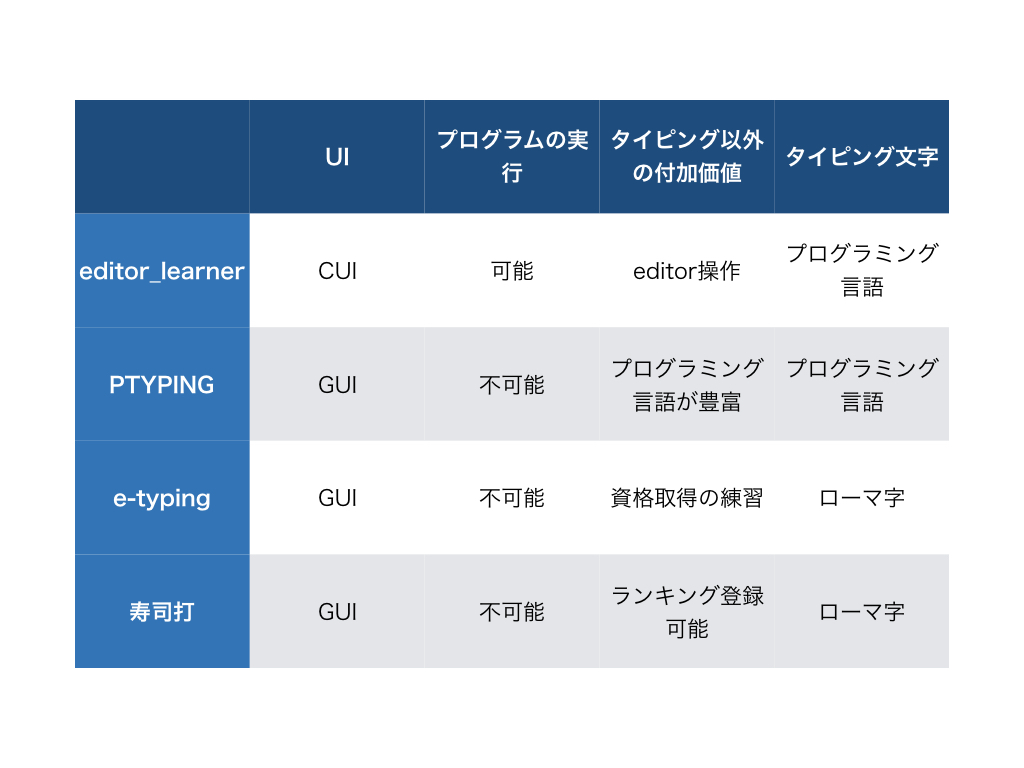
\includegraphics[width=150mm]{../../picture/compare.jpeg}
\end{center}
\caption{他のソフトとの比較.\label{compare}}

\label{fig:}
\end{figure}

上記のタイピングソフトは自分もよく使っていたタイピングソフトであり,評価も高いソフトである.それぞれの特徴は以下の通り,

\section{PTYPING}\label{ptyping}

PTYPINGは豊富なプログラム言語が入力可能である.しかし,コードを打つのではなく,コードに使われるintなどよく使われる単語が60秒の間にどれだけ打てるかというソフトです.

\section{e-typing}\label{e-typing}

e-typingはインターネットで無料提供されているソフトである.ローマ字入力を基本として,単語,短文,長文の3部構成となっておりタイピングの資格取得の練習もできる.

\section{寿司打}\label{ux5bffux53f8ux6253}

自分が一番利用したサイト,GUIベースによりローマ字入力を基本とし,打てば打つほど秒数が伸びていきどれだけ入力できるかをランキング形式で表示される.

\section{考察}\label{ux8003ux5bdf}

これら全てのソフトを利用した結果,editor\_learnerはローマ字入力ができない点では他のソフトに遅れをとるが,実際にプログラムを書くようになってからコードを写経することで\{\}や()などといったローマ字入力ではあまり入力しないような記号の入力が非常に早くなった.さらに,editor\_learnerは現段階ではRubyの学習のみだが,引数を変えて元となるプログラムを作成することで全てのプログラム言語を学ぶことができる.さらに,実際にコードを入力することができるソフトはたくさんあるが,実行可能なものは少ない(Webで行うものが大半を占めているから.)実際に西谷研究室でeditor\_learnerで学習を行っていない学生と行った自分のrandom\_check平均秒数は前者は200秒程なのに対して,自分は60秒程である.これらの結果からeditor\_learnerによる学習により,Ruby言語の学習にもなり,タイピング速度,正確性の向上,CUI操作の適応による差が出たと考えた.

    